\chapter{Limit}
The events passing the kinematical selection are compared with expectations
from Standard Model background sources. The number of expected events from
the signal Monte Carlo is shown in table~\ref{tab:signal_yields}. The
backgrounds are compared to the observed event yields in
table~\ref{tab:background_yields}.
        \begin{table}[pbt]
            \centering
            \begin{tabular}{l *3{r@{$\pm$}l}}
                
\toprule
dataset & \multicolumn{2}{c}{same-sign, 2 jets}& \multicolumn{2}{c}{preselection}& \multicolumn{2}{c}{razor} \\
\midrule
T53 400& 211.10 & 10.73& 151.16 & 7.73& 54.34 & 2.88\\
T53 450& 104.52 & 5.31& 77.93 & 3.98& 41.34 & 2.15\\
T53 500& 52.76 & 2.68& 40.09 & 2.04& 25.61 & 1.32\\
T53 550& 28.53 & 1.45& 22.47 & 1.14& 16.22 & 0.83\\
T53 600& 15.34 & 0.78& 12.07 & 0.61& 9.39 & 0.48\\
T53 650& 8.65 & 0.44& 6.87 & 0.35& 5.57 & 0.28\\
T53 700& 5.00 & 0.25& 3.98 & 0.20& 3.37 & 0.17\\
T53 750& 2.97 & 0.15& 2.35 & 0.12& 2.01 & 0.10\\
 \\
\bottomrule

            \end{tabular}
            \caption{Signal Monte Carlo yields for the various mass points
            in the three decay channels. Statistical and systematic uncertainties are shown.}
            \label{tab:signal_yields_sum}
        \end{table}


        \begin{table}[pbt]
            \centering
            \begin{tabular}{l *3{r@{$\pm$}l}}
                
\toprule
dataset & \multicolumn{2}{c}{same-sign, 2 jets}& \multicolumn{2}{c}{preselection}& \multicolumn{2}{c}{razor} \\
\midrule
WW, WWW& 2.86 & 6.67& 0.22 & 0.45& 0.05 & 0.14\\
TTZ, TTW& 3.97 & 9.31& 1.33 & 3.20& 0.31 & 0.71\\
WZ, ZZ& 8.57 & 6.17& 0.41 & 0.36& 0.09 & 0.08\\
\midrule
total MC& 15.40 & 13.01& 1.95 & 3.25& 0.45 & 0.73\\
charge misid& 18.38 & 4.81& 0.22 & 0.17& 0.04 & 0.03\\
non-prompt & 34.99 & 1.91& 2.27 & 0.48& 0.12 & 0.11\\
observed & \multicolumn{2}{c}{77}& \multicolumn{2}{c}{3}& \multicolumn{2}{c}{2} \\
\bottomrule

            \end{tabular}
            \caption{Expected backgrounds and observed yields for different
            cuts in the \E\E\ channel. Statistical and systematic uncertainties are
            shown.}
            \label{tab:background_yields_ee}
        \end{table}

        \begin{table}[pbt]
            \centering
            \begin{tabular}{l *3{r@{$\pm$}l}}
                
\toprule
dataset & \multicolumn{2}{c}{same-sign, 2 jets}& \multicolumn{2}{c}{preselection}& \multicolumn{2}{c}{razor} \\
\midrule
WW, WWW& 6.63 & 6.67& 0.48 & 0.45& 0.16 & 0.14\\
TTZ, TTW& 9.13 & 9.31& 3.39 & 3.20& 0.71 & 0.71\\
WZ, ZZ& 17.45 & 6.17& 1.12 & 0.36& 0.19 & 0.08\\
\midrule
total MC& 33.21 & 13.01& 4.99 & 3.25& 1.07 & 0.73\\
charge misid& 4.66 & 4.81& 0.60 & 0.17& 0.11 & 0.03\\
non-prompt & 50.61 & 3.41& 5.44 & 1.20& 0.25 & 0.28\\
observed & \multicolumn{2}{c}{48}& \multicolumn{2}{c}{8}& \multicolumn{2}{c}{2} \\
\bottomrule

            \end{tabular}
            \caption{Expected backgrounds and observed yields for different
            cuts in the \E\M\ channel. Statistical and systematic uncertainties are
            shown.}
            \label{tab:background_yields_emu}
        \end{table}

        \begin{table}[pbt]
            \centering
            \begin{tabular}{l *3{r@{$\pm$}l}}
                
\toprule
dataset & \multicolumn{2}{c}{same-sign, 2 jets}& \multicolumn{2}{c}{preselection}& \multicolumn{2}{c}{razor} \\
\midrule
WW, WWW& 3.78 & 6.67& 0.18 & 0.45& 0.07 & 0.14\\
TTZ, TTW& 5.47 & 9.31& 1.68 & 3.20& 0.39 & 0.71\\
WZ, ZZ& 8.60 & 6.17& 0.45 & 0.36& 0.14 & 0.08\\
\midrule
total MC& 17.86 & 13.01& 2.31 & 3.25& 0.60 & 0.73\\
charge misid& 1.01 & 4.81& 0.01 & 0.17& 0.00 & 0.03\\
non-prompt & 19.64 & 2.06& 3.59 & 0.89& 0.39 & 0.28\\
observed & \multicolumn{2}{c}{32}& \multicolumn{2}{c}{4}& \multicolumn{2}{c}{0} \\
\bottomrule

            \end{tabular}
            \caption{Expected backgrounds and observed yields for different
            cuts in the \M\M\ channel. Statistical and systematic uncertainties are
            shown.}
            \label{tab:background_yields_mumu}
        \end{table}

        \begin{table}[pbt]
            \centering
            \begin{tabular}{l *3{r@{$\pm$}l}}
                
\toprule
dataset & \multicolumn{2}{c}{same-sign, 2 jets}& \multicolumn{2}{c}{preselection}& \multicolumn{2}{c}{razor} \\
\midrule
WW, WWW& 13.28 & 6.67& 0.88 & 0.45& 0.28 & 0.14\\
TTZ, TTW& 18.57 & 9.31& 6.39 & 3.20& 1.41 & 0.71\\
WZ, ZZ& 34.62 & 6.17& 1.97 & 0.36& 0.42 & 0.08\\
\midrule
total MC& 66.47 & 13.01& 9.25 & 3.25& 2.12 & 0.73\\
charge misid& 24.05 & 4.81& 0.83 & 0.17& 0.15 & 0.03\\
non-prompt & 105.24 & 52.80& 11.30 & 5.86& 0.76 & 0.56\\
observed & \multicolumn{2}{c}{157}& \multicolumn{2}{c}{15}& \multicolumn{2}{c}{4} \\
\bottomrule

            \end{tabular}
            \caption{Expected backgrounds and observed yields for different
            cuts in the three decay channels. Statistical and systematic uncertainties are
            shown.}
            \label{tab:background_yields_sum}
        \end{table}

No significant excess over the SM expectations is observed, and we can set
lower bounds on the masses of the top partners.

Exclusion limits are computed at the 95\% confidence level for an event
counting experiment. The event yields from the three decay channels are
combined when setting the limits. The limit is computed using the CLs method
and an LHC-style profile likelihood. Poisson statistics are used to model
the signal and gaussian distributions are used for integrating over nuisance
parameters. The expected and observed limits are shown in
figure~\ref{fig:limit}.
The expected limit is~\unit[658]{GeV}, the observed limit
is~\unit[633]{GeV}.

\begin{figure}[htb]
    \centering
    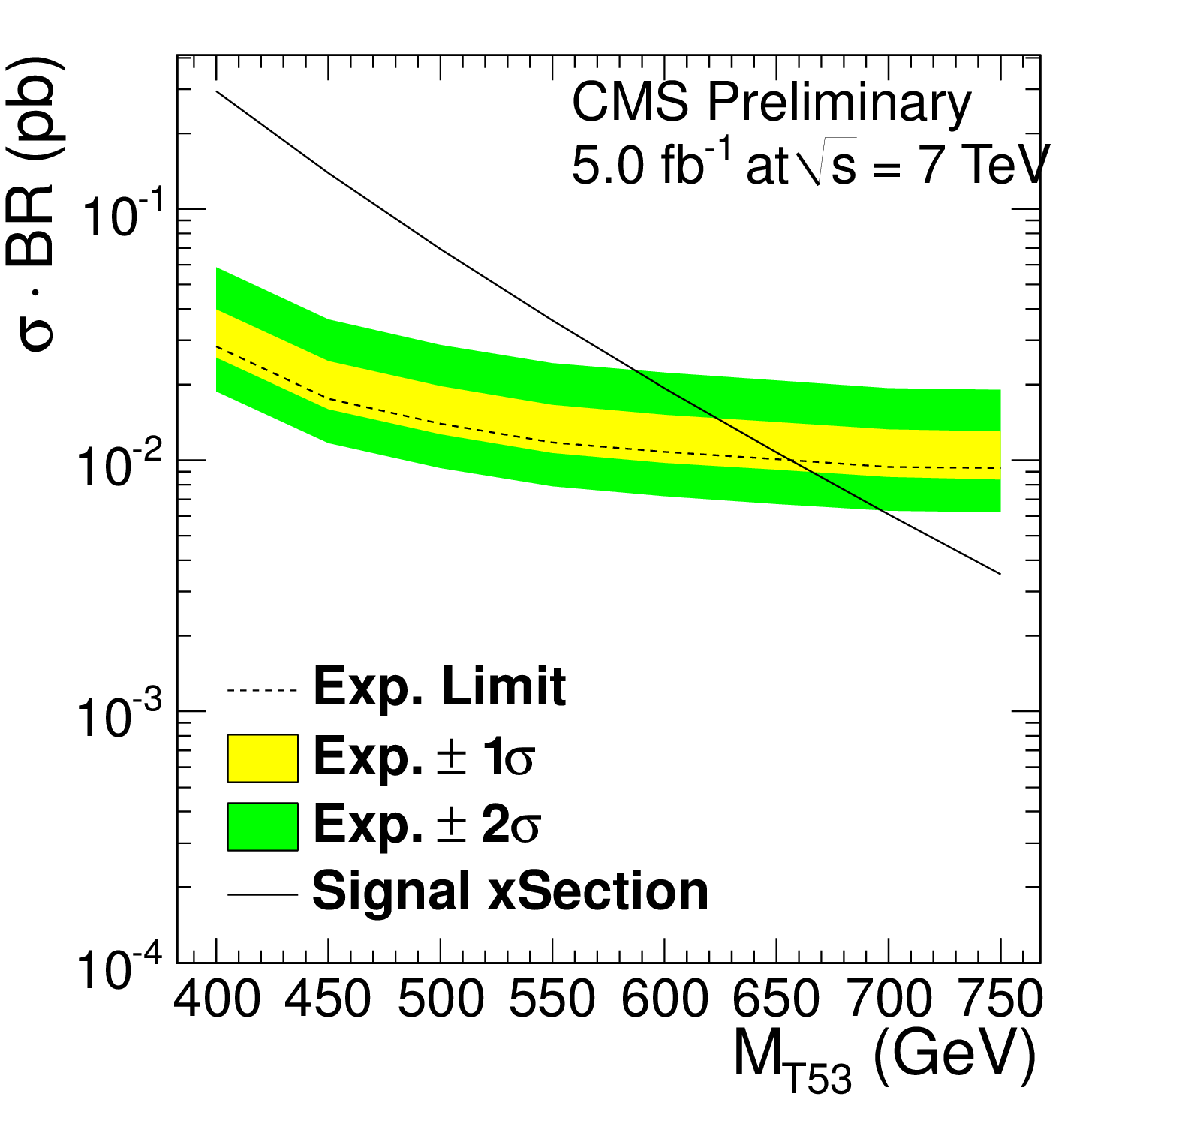
\includegraphics[width=.9\textwidth]{images/pdf/oLimit_limit_macro_4jets_opt_btag_200_350_02}

    \caption{Observed and expected limits for the production cross sections
    of the top partners.}
    \label{fig:limit}
\end{figure}
